\begin{sidewaysfigure}
    \centering
    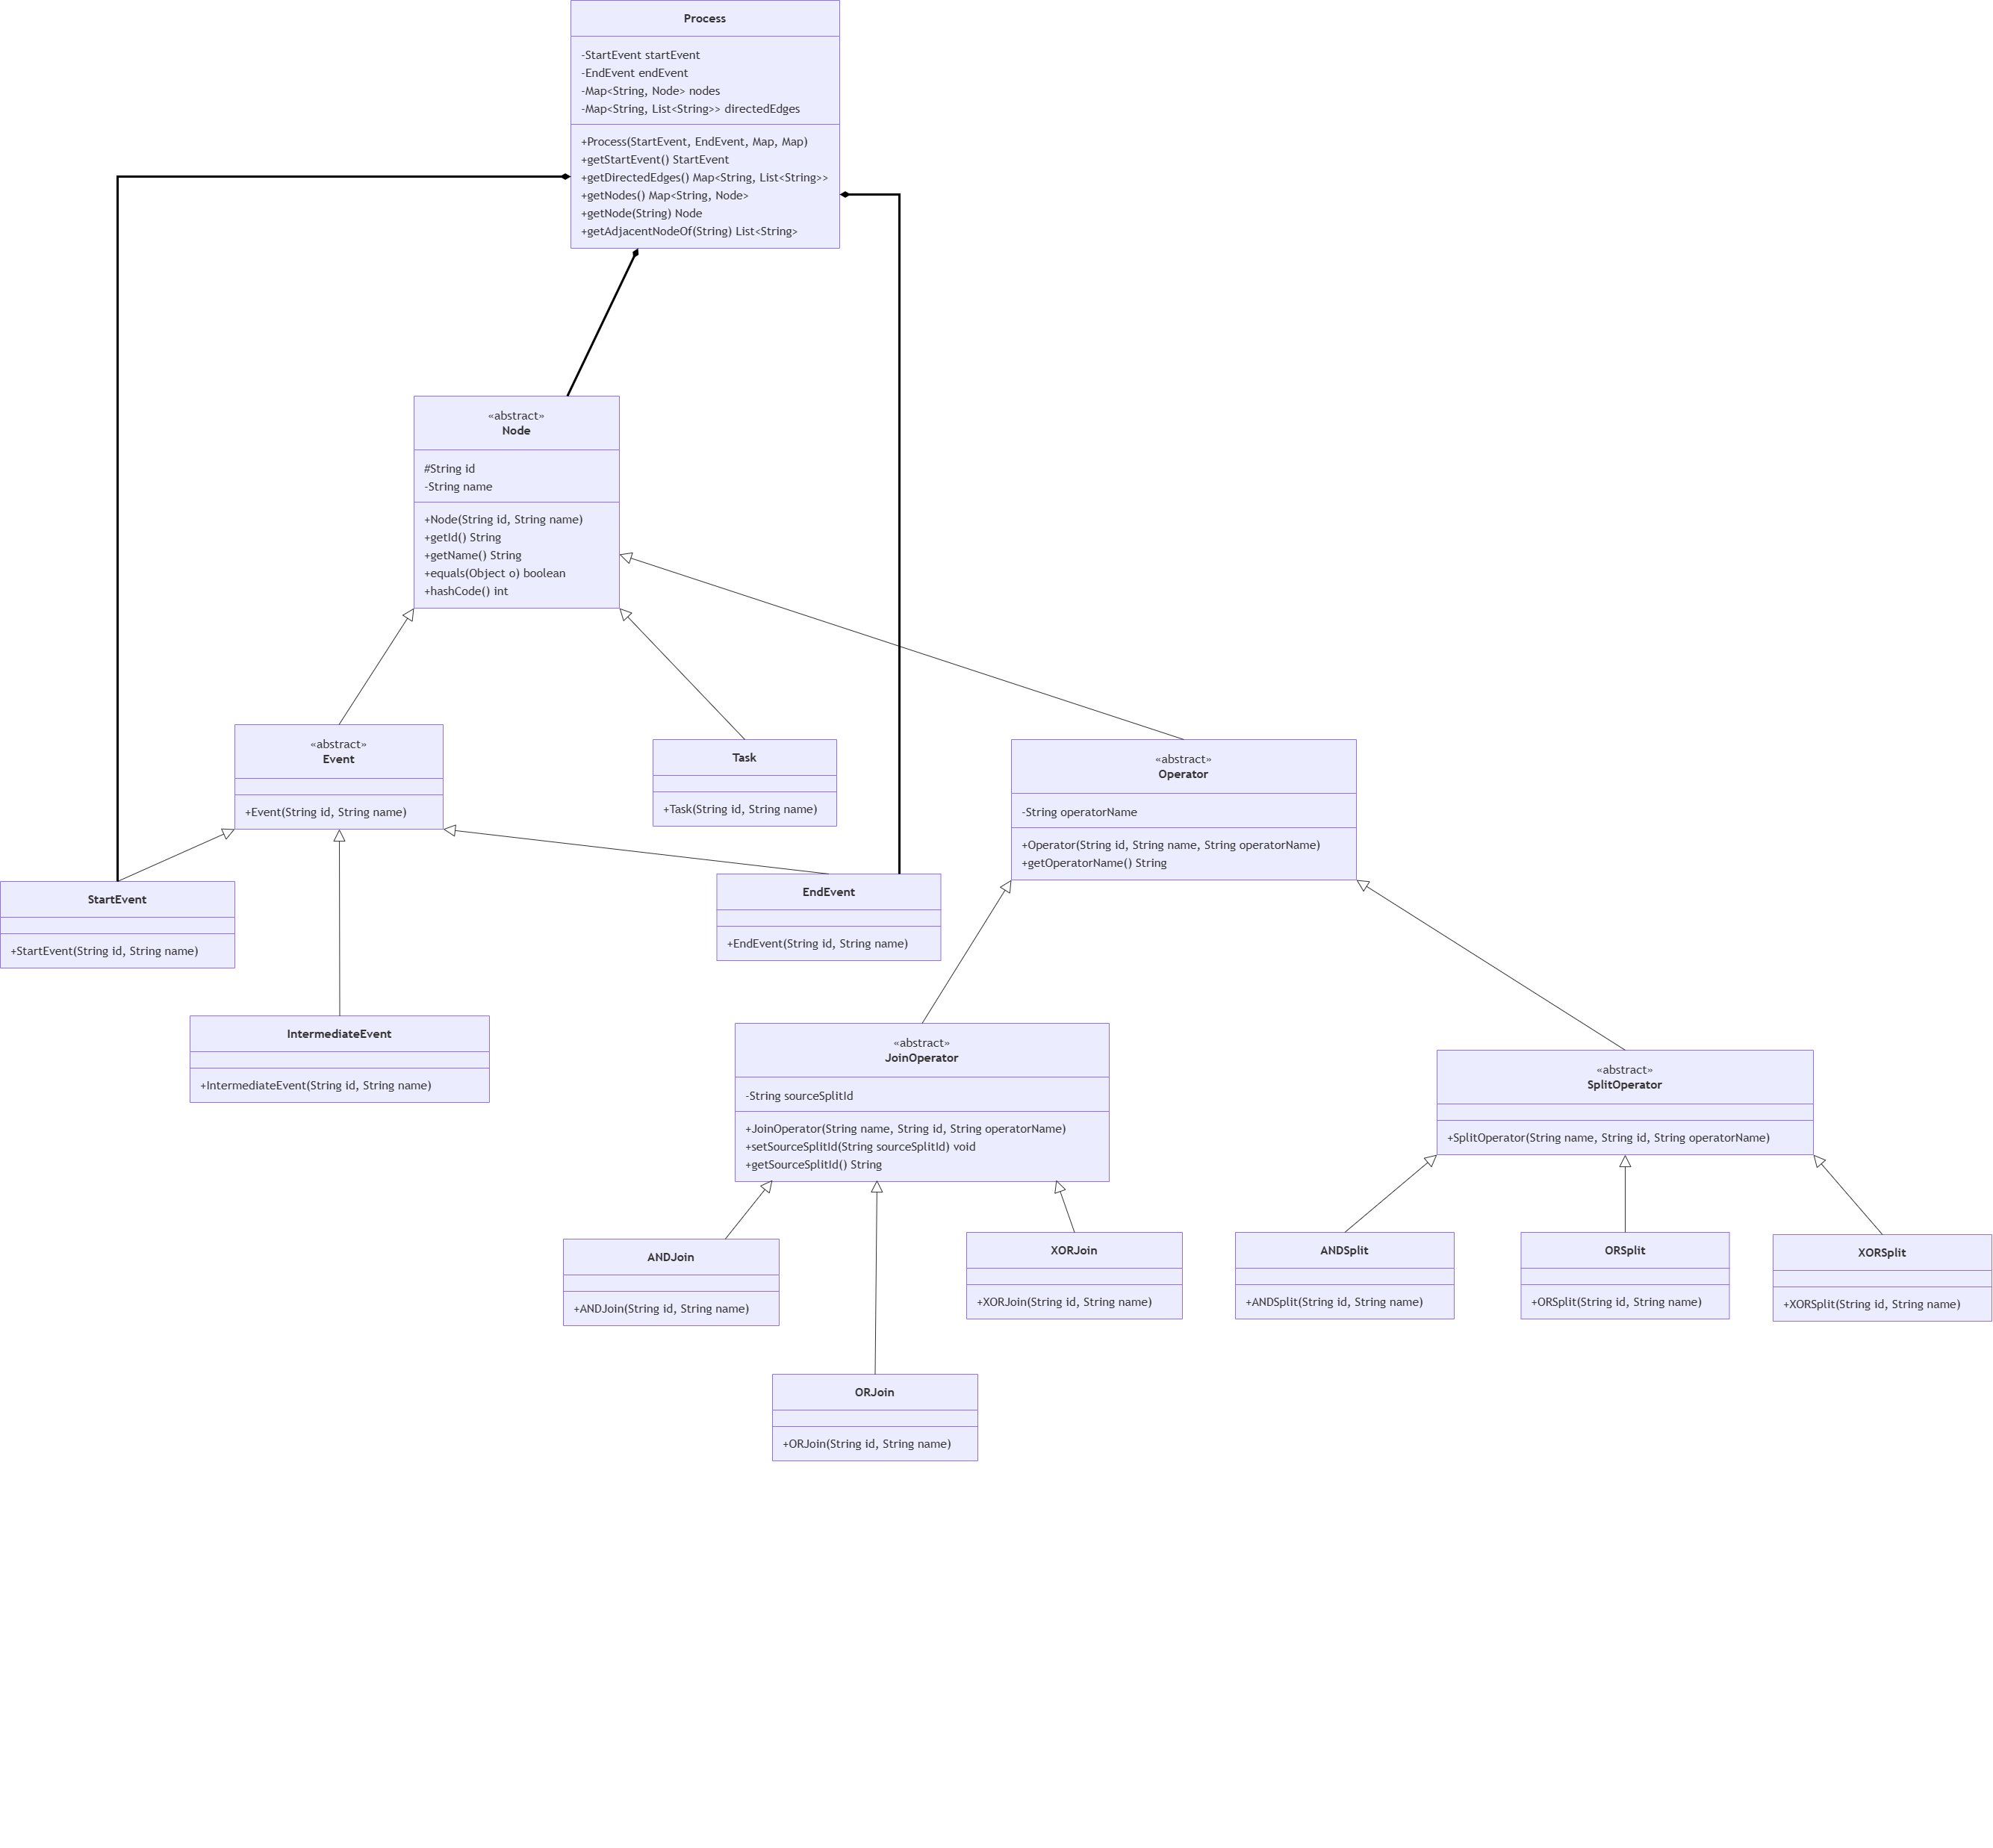
\includegraphics[width=\textwidth]{Graphics/Prozess-UML.png}
    \caption{UML Diagramm der Prozessmodellimplementierung}
    \label{fig:prozess-uml}
\end{sidewaysfigure}

\begin{sidewaysfigure}
    \centering
    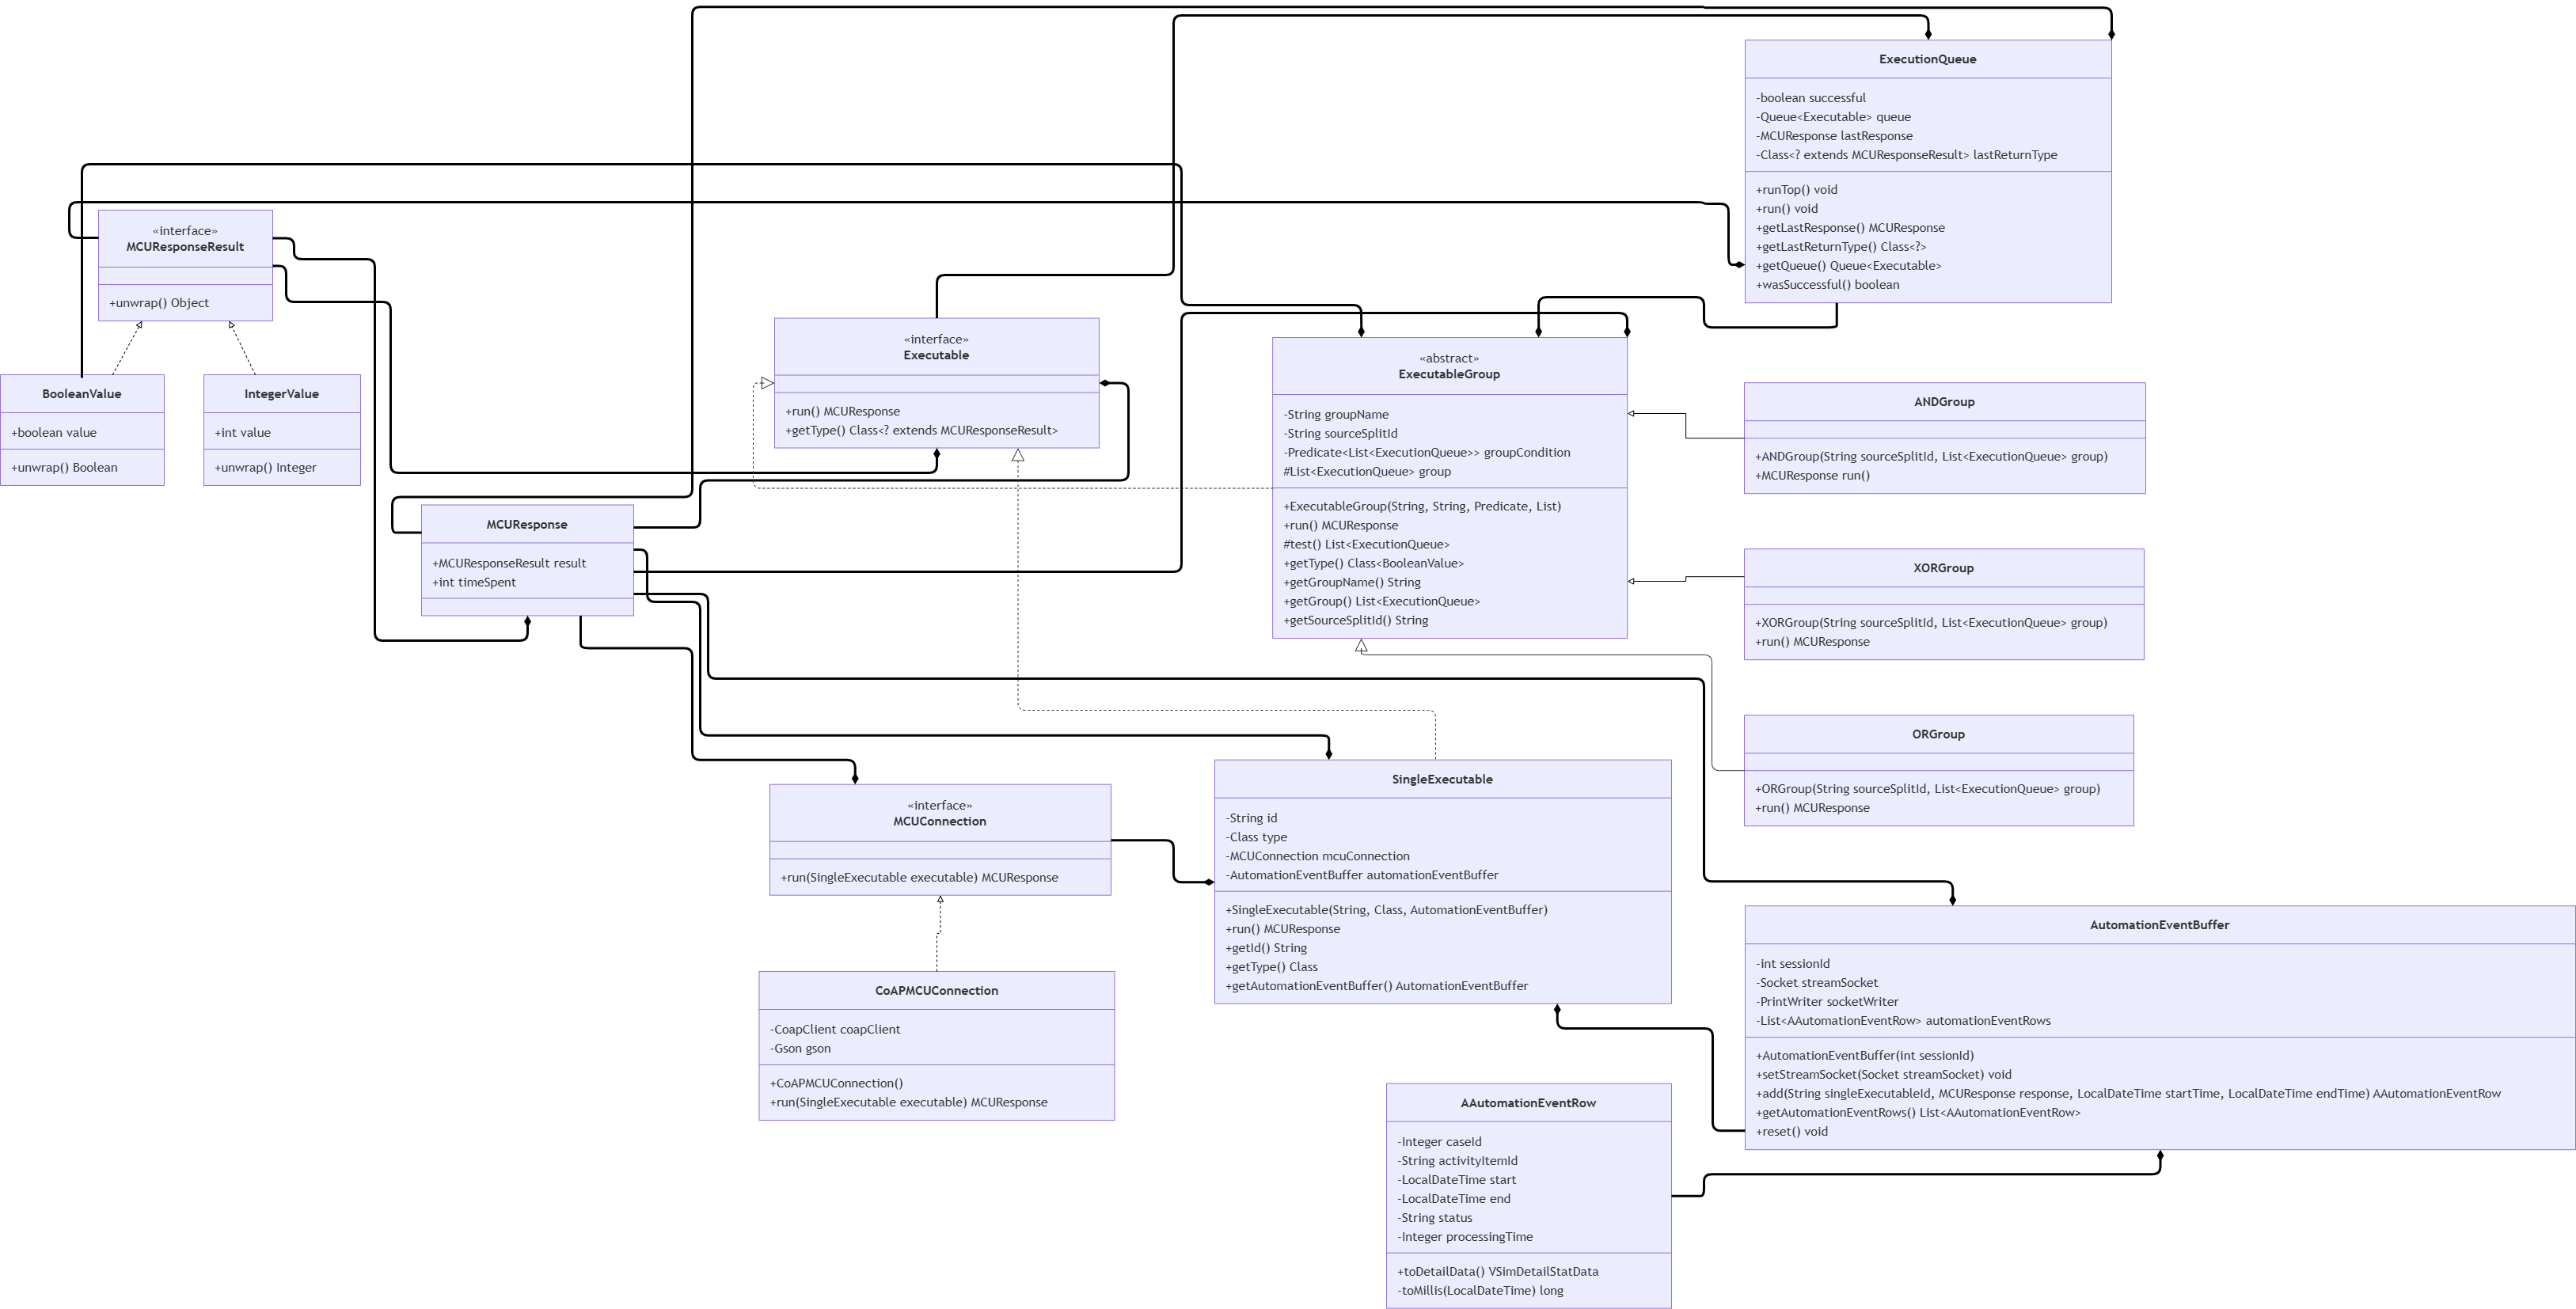
\includegraphics[width=\textwidth]{Graphics/Ausführungsmodell-UML.png}
    \caption{UML Diagramm des Ausführungsmodellimplementierung}
    \label{fig:executable-uml}
\end{sidewaysfigure}

\begin{sidewaysfigure}
    \centering
    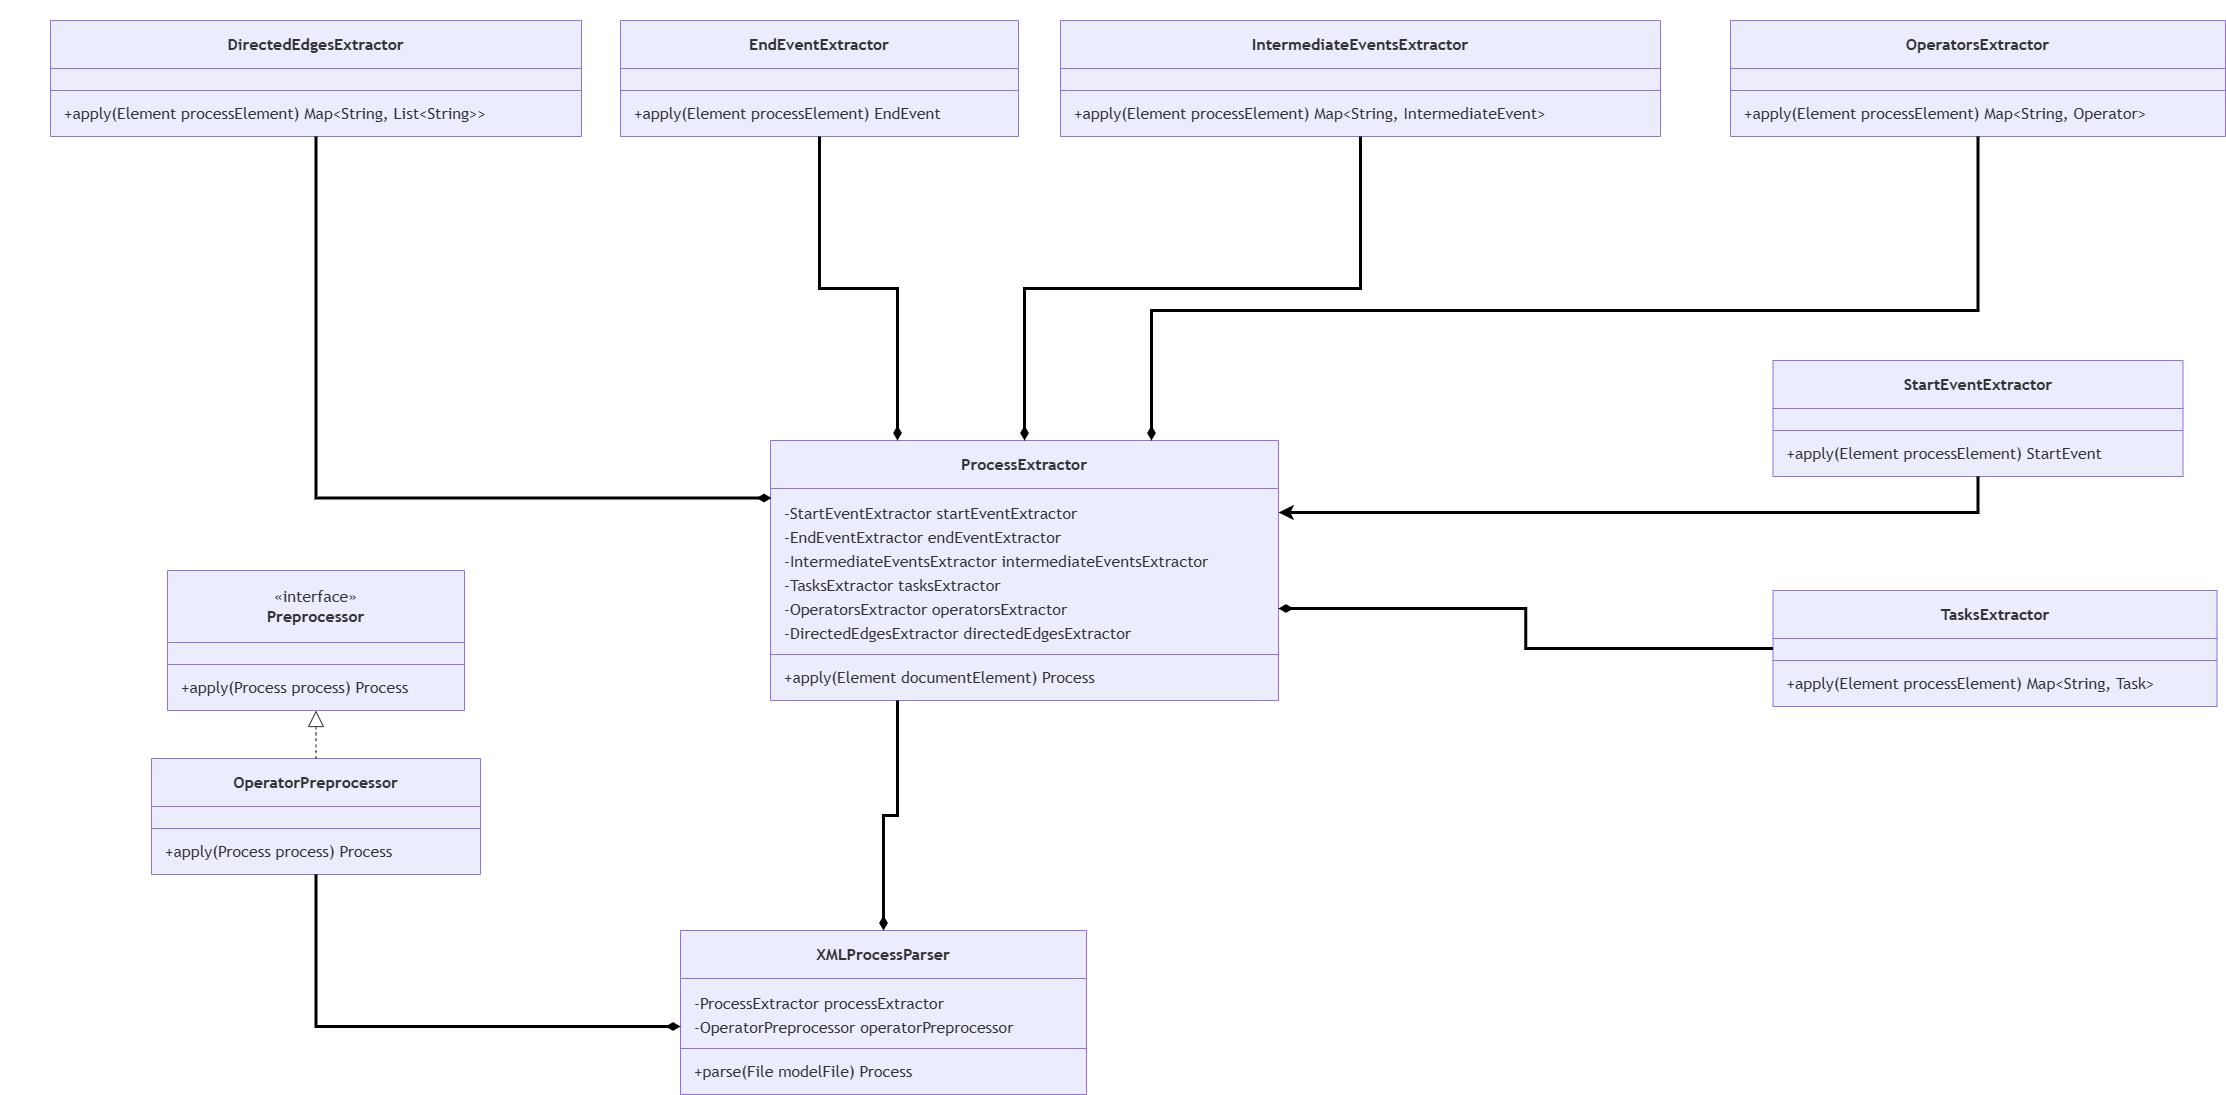
\includegraphics[width=\textwidth]{Graphics/Process-Builder-UML.png}
    \caption{UML Diagramm des Prozessmodellkonstruktionsklassen}
    \label{fig:process-builder-uml}
\end{sidewaysfigure}

\begin{sidewaysfigure}
    \centering
    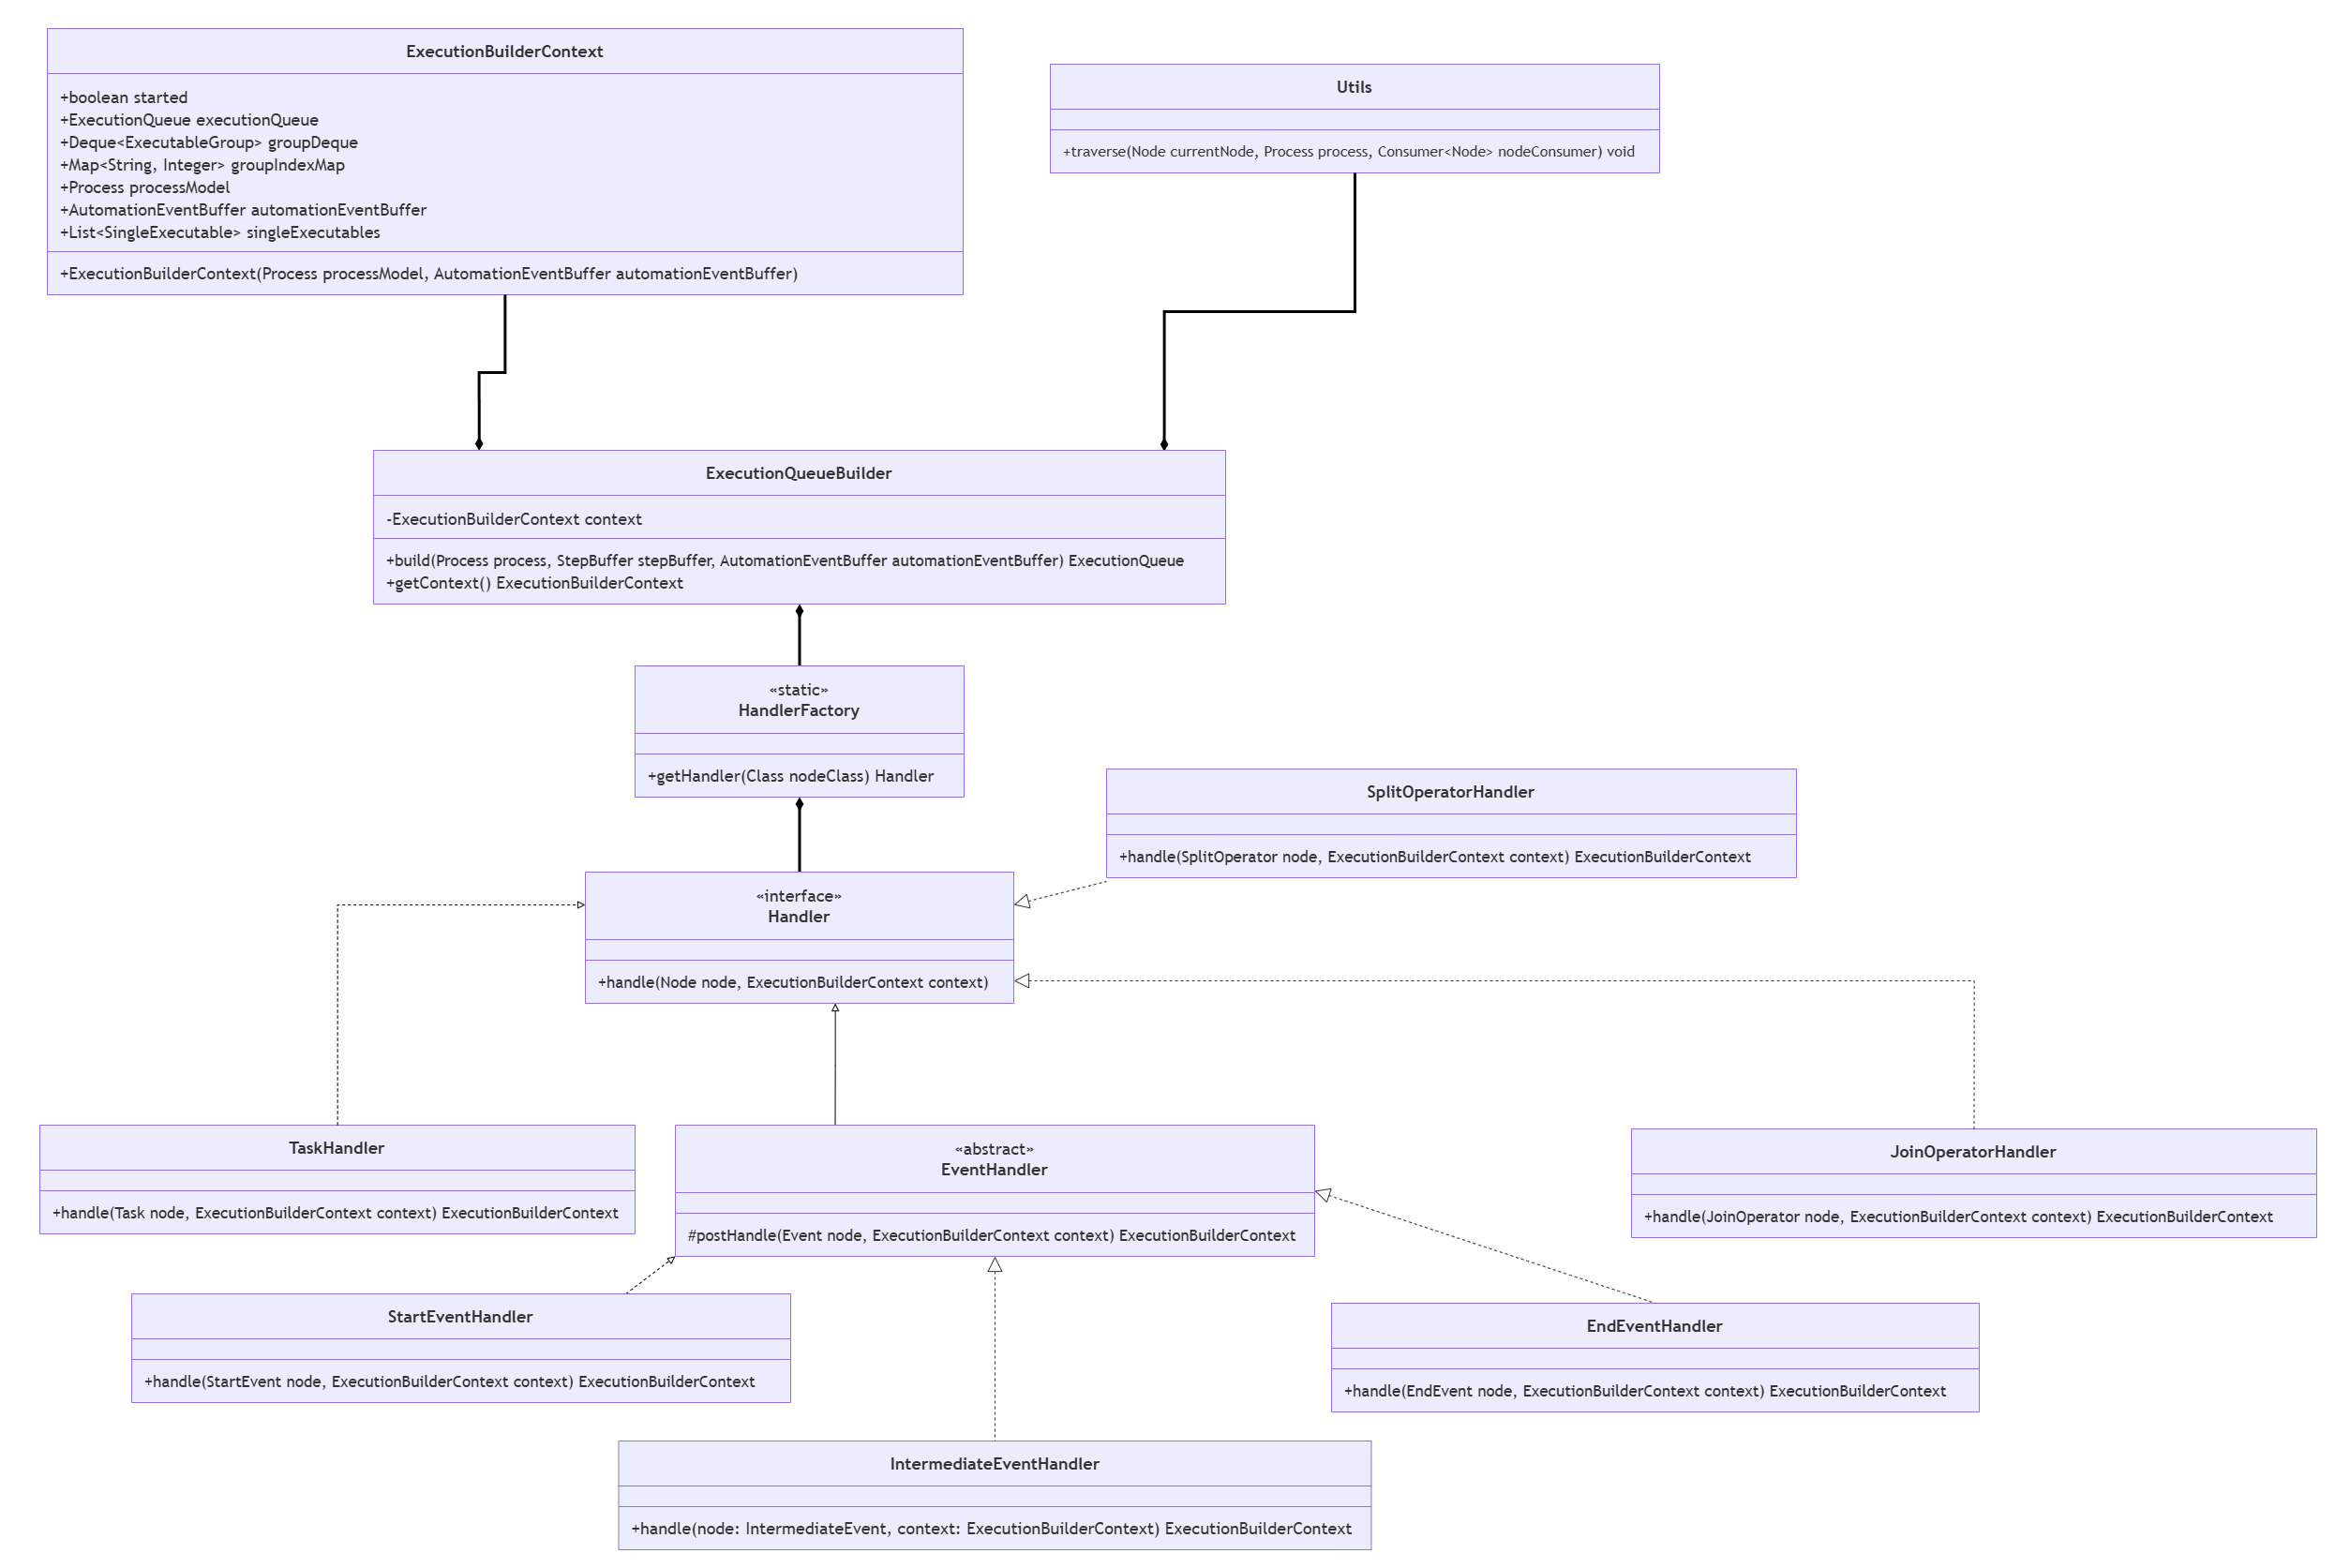
\includegraphics[width=\textwidth, height=\textheight, keepaspectratio]{Graphics/EPK-Compiler-UML.png}
    \caption{UML Diagramm des EPK-Compilers}
    \label{fig:epk-compiler-uml}
\end{sidewaysfigure}

\begin{figure}
    \centering
    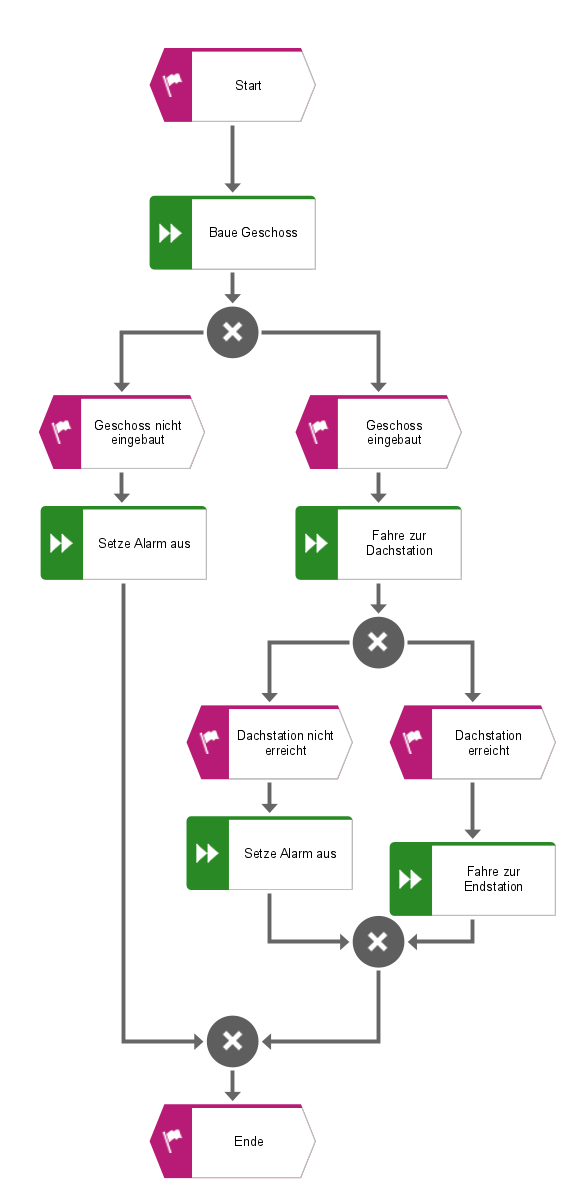
\includegraphics[width=\textwidth]{Graphics/Bauklötzchenhaus-EPK-2.png}
    \caption{EPK-Diagramm des Prozessess eines Hausbaus mit Bauklötzchenhauses}
    \label{fig:brick-house-epk}
\end{figure}